%%%%%%%%%%%%%%%%%%%%%%%%%%%%%%%%%%%%%%%%%%%%%%%%%%%%%%%%%%%%%%%%%%%%%%%%%%%%%%%%
%2345678901234567890123456789012345678901234567890123456789012345678901234567890
%        1         2         3         4         5         6         7         8

\documentclass[letterpaper, 10 pt, conference]{ieeeconf}  % Comment this line out if you need a4paper

%\documentclass[a4paper, 10pt, conference]{ieeeconf}      % Use this line for a4 paper

\IEEEoverridecommandlockouts                              % This command is only needed if 
                                                          % you want to use the \thanks command

\overrideIEEEmargins                                      % Needed to meet printer requirements.

%In case you encounter the following error:
%Error 1010 The PDF file may be corrupt (unable to open PDF file) OR
%Error 1000 An error occurred while parsing a contents stream. Unable to analyze the PDF file.
%This is a known problem with pdfLaTeX conversion filter. The file cannot be opened with acrobat reader
%Please use one of the alternatives below to circumvent this error by uncommenting one or the other
%\pdfobjcompresslevel=0
%\pdfminorversion=4

% See the \addtolength command later in the file to balance the column lengths
% on the last page of the document

% The following packages can be found on http:\\www.ctan.org
%\usepackage{graphics} % for pdf, bitmapped graphics files
%\usepackage{epsfig} % for postscript graphics files
%\usepackage{mathptmx} % assumes new font selection scheme installed
%\usepackage{times} % assumes new font selection scheme installed
%\usepackage{amsmath} % assumes amsmath package installed
\usepackage{amssymb}  % assumes amsmath package installed
\usepackage{amscd,amsmath}
\usepackage{amsfonts}
\usepackage{biblatex}
\usepackage{csvsimple}
\usepackage{pgfplots}
\pgfplotsset{compat=1.7}
\usepackage{graphicx}
\usepackage{import}
\usepackage{placeins}

\title{\LARGE \bf
Fault Detection to Increase Reliability of Kalman Filter for Satellite Attitude Determination
}


\author{Louw UJ$^{1}$, Jordaan HW$^{2}$, Schoeman JC$^{3}$% <-this % stops a space
\thanks{*This work was not supported by any organization}% <-this % stops a space
\thanks{$^{1}$Louw UJ is with Faculty of Electronic \& Electrical Engineering, Electronic System            Laboratory, University of Stellenbosch, Stellenbosch Central, Stellenbosch, 7600
        {\tt\small louwuj@gmail.com}}%
}

\addbibresource{bibliography.bib} 

\begin{document}



\maketitle
\thispagestyle{empty}
\pagestyle{empty}


%%%%%%%%%%%%%%%%%%%%%%%%%%%%%%%%%%%%%%%%%%%%%%%%%%%%%%%%%%%%%%%%%%%%%%%%%%%%%%%%
\begin{abstract}

The Kalman Filter is a state estimator that is often used in attitude determination of satellites. A Kalman filter is highly sensitive to anomalies that occur in sensors. A good example of this is the reflection of a solar panel on a sun sensor that changes the perceived sun vector. This in term influences the estimation of the attitude by the kalman filter and consequently the control of the satellite. Detecting anomalies in sensors and omitting the sensor reading from the measurement update of the Kalman Filter could increase the stability and reliability of the Kalman filter for satellite attitude determination.

\end{abstract}


%%%%%%%%%%%%%%%%%%%%%%%%%%%%%%%%%%%%%%%%%%%%%%%%%%%%%%%%%%%%%%%%%%%%%%%%%%%%%%%%
\section{INTRODUCTION}
The Extended Kalman filter... Various prediction methodologies... Various sensor anomalies... (specific anomalies such as solar reflection).

\section{Related Work}


\subsection{Extended Kalman Filter}
Explanation of EKF for attitude estimation.

\subsection{Sensitivity of Kalman Filter}
The effect of sensor anomalies on kalman filter.

\section{Sensor anomalies}
List of sensor anomalies and a model of specific anomalies. (solar panel reflection)

\subsection{Reflection}`
Previous work done by \textcite{Cilden-Guler2021} provides models that determine albedo effects from the earth and adjust the CSS measurements to improve accuracy.
Model of Reflection with pgfplots.

\begin{figure}[!htb]
	\centering
	\def\svgwidth{7cm}
	\import{Figures/}{ReflectionModel.pdf_tex}
	\caption{Cube Sat}
	\label{fig:Reflection}
\end{figure}

\begin{figure}[!htb]
	\centering
	\def\svgwidth{7cm}
	\import{Figures/}{ReflectionModelPoints.pdf_tex}
	\caption{Reflection}
	\label{fig:ReflectionPoints}
\end{figure}

The assumption is made that the solar panel can be modelled as a simple plane. Therefore light that hits the solar panel will reflect as if it hits a perfectly smooth mirror. It is also assumed that if any reflection from the solar panel hits the sun sensor, the sun sensor will then default to the reflection ray instead of the modelled sun vector. 

To model reflection from the solar panels to the sun sensor only two corners of the solar panel and two corners of the sun sensor can be taken into account. From Figure~\ref{fig:ReflectionPoints} it is evident that if the solar panel reflects on corner $y$ that corner $x$ will also receive light from the reflection. The same is true for corner $z$ and $w$. Since $C'$ will be at the exact same position as $C$, the reflection from the sun does not need to be calculated for $C$, this is also true for $D$. Therefor it is only necessary to calculate the reflected positions $A'$ and $B'$.

The reflected position $A'$ can be calculated as the intersection of the reflected vector $RR'$ with plane $xyzw$. We also know the position of $A$ and from this the exact position of $A'$ can be calculated as

\begin{equation}
A' = A
\end{equation}

\section{Anomaly Detection}
To be able to recover from sensor anomalies or to exclude the sensor from the kalman filter, the anomaly must be detected and the sensor from which the anomaly in the data occurs must be classified.

\subsection{Detection}
The first step to implementing a FDIR for kalman filter robustness is to detect whether an anomaly has occured on one of the filters. There are various different methods for fault detection, with both supervised and unsupervised methods. However this study will only focus on a single method proposed by \textcite{DeSilva2020} to detect failures in sensors.

The proposed method by \textcite{DeSilva2020} uses Dynamic Mode Decomposition (DMD), which was originally developed by \textcite{schmid2011applications} and further expanded to include control by \textcite{proctor2016dynamic}, to provide an estimation of a sensor vector based on the previous measurement fo the sensor as well as the measurements of the other sensors in the system. DMD was first developed in the fluids community and constructs a matrix $\mathbf{A}$ to relate the state vector $x$ with the following time step of the state vector, $x_{k+1}$. The state vector in our case will be the measurement vector of the specific sensor that we want to monitor.
\begin{equation}
	x_{k+1} = \mathbf{A}x_k
\end{equation}
Where $x_k$ and $x_{k+1}$ over a time period will be denoted as $\mathbf{X}$ and $\mathbf{X'}$ respectively.

The method of DMD however is useful for high order systems where the calculation of $\mathbf{A}$ is computation intensive. This is not the case for our system and using DMD is not justifiable. Therefore we calculate the pseudo-inverse of $\mathbf{X}$, denote it as $\mathbf{X^{\dagger}}$, and $\mathbf{A}$ can be calculate as
\begin{equation}
	\mathbf{A} = \mathbf{X}\mathbf{X^{\dagger}}
\end{equation}
This necessitates the required data for the state vector. The article by \textcite{DeSilva2020} however includes the $\mathbf{B}$ to relate the vector measurements of the other sensors to adjust the predicted state, $x_{k+1}$ of the monitored sensor. 
\begin{equation}
	x_{k+1} = \boldsymbol{A}x_k + \boldsymbol{B}y_k
	\label{control DMD}
\end{equation}
Where $y_k$ is the other sensor measurements. This is adjusted for our use case, where $y_k$ is the control inputs for the magnetotorquers and reaction wheels and $x_k$ is all of the sensor measurements. Consequently, the model of \ref{control DMD} denotes the prediction of the sensor measurements in time step $k+1$ based on the current sensor measurements and control inputs.
Thereafter, as implemented by \textcite{DeSilva2020} the model is adjusted by with a Kalman Filter. From $\boldsymbol{A}$ and $\boldsymbol{B}$ the Kalman filter can be implemented to predict $x_{k+1}$
\begin{equation}
	\hat{x}_{k+1} = A\hat{x}_k + By_k + K(x_k - \hat{x}_k)
\end{equation}
After  the calculation of $\hat{x}_{k+1}$ \textcite{DeSilva2020} proposes a moving average of the innovation covariance
\begin{equation}
	\boldsymbol{V}_k = \frac{1}{N} \sum_{i=k-N}^k (x_i - \hat{x}_i)(x_i - \hat{x}_i)^T
\end{equation}
The moving average is used as an additional input parameter to a decision tree that classifies binary anomalies based on the $\boldsymbol{x_k}$. According to

Decision Tree (Discuss gini index)

\begin{equation}
GI = 1 - \sum_{i = 1}^{n}{(P_i)^2}
\end{equation}

\begin{figure}[!htb]
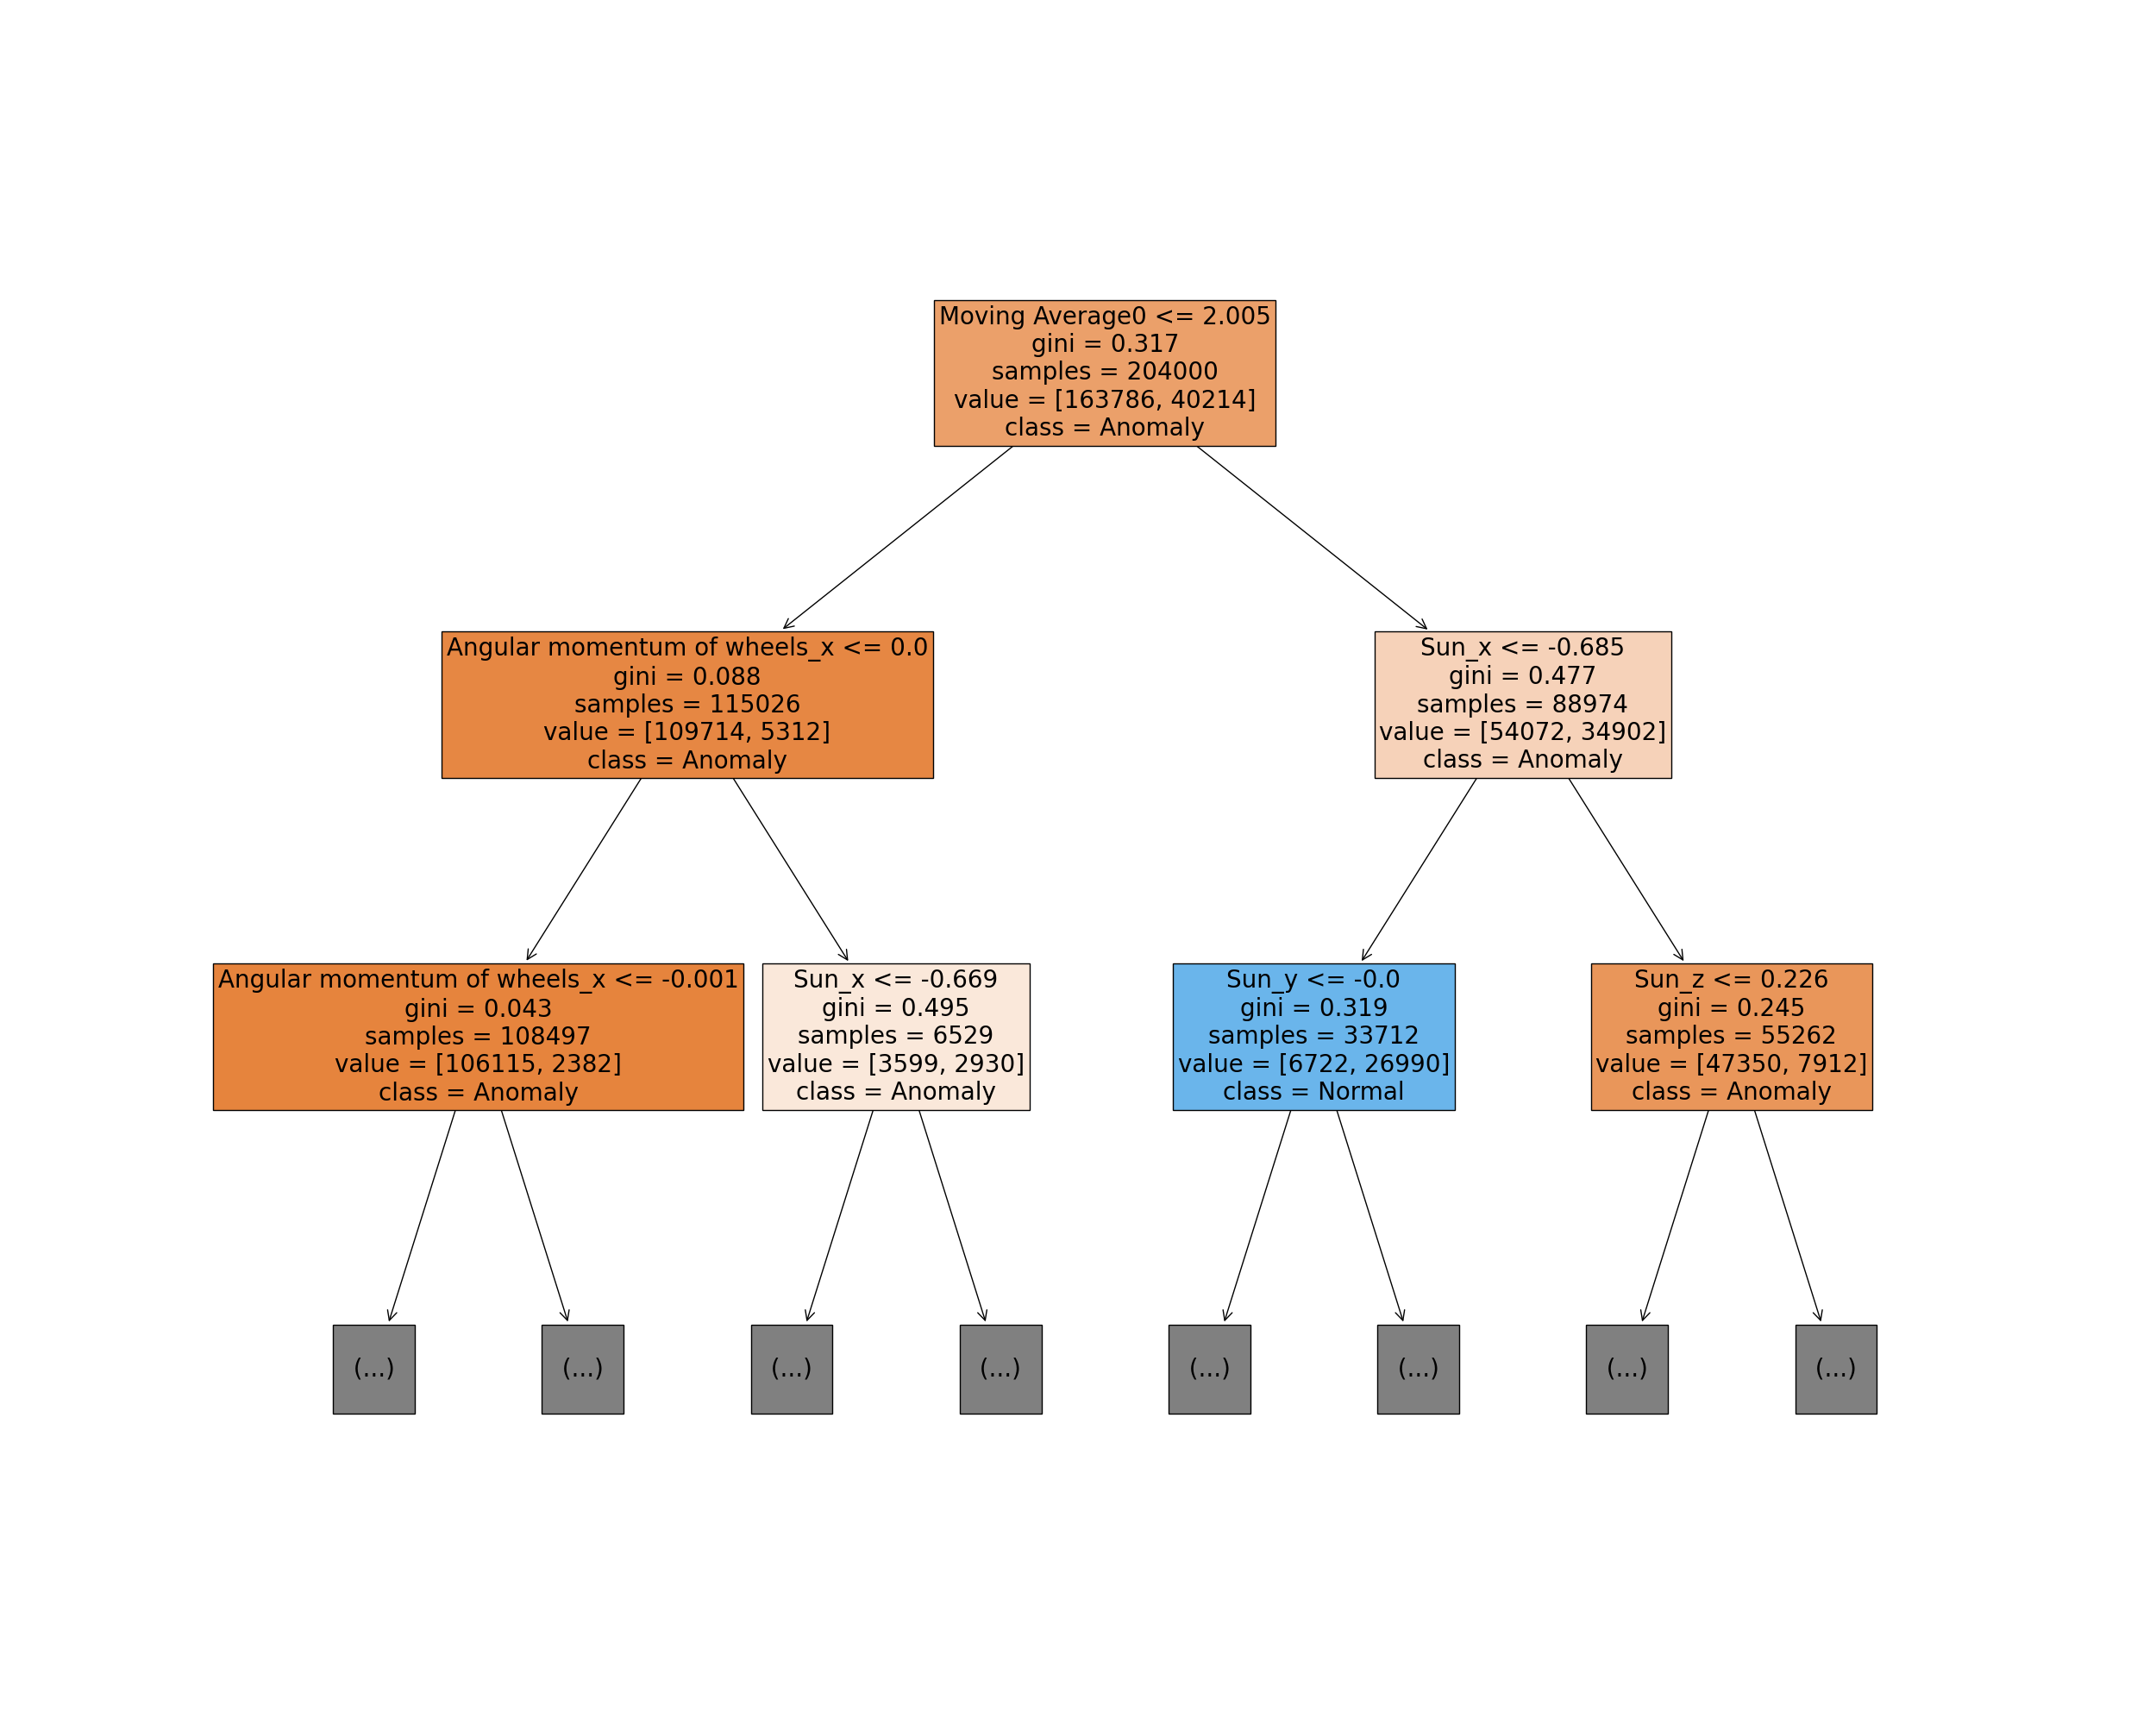
\includegraphics[width = 7cm]{/home/ulrich/Documents/Masters thesis/Satellite/Hyperparameters/PhysicsEnabledDMDMethod/DecisionTreeBinaryClass.png}
\end{figure}

\subsection{Isolation}
Decision tree or any other multi-classifying method.

\begin{figure}[!htb]
\includegraphics[width = 7cm]{/home/ulrich/Documents/Masters thesis/Satellite/Hyperparameters/PhysicsEnabledDMDMethod/DecisionTreeMultiClass.png}
\end{figure}


\subsection{Recovery}
Backtracking on kalman filter... Removing sensor measurement update... If a fault is predicted, the estimated vector model from the kalman filter is used to to determine the reference position for the control as well as the calculations for the control.

\section{Testing methodology}
Simulation... Induce anomalies based on physical models or at a specified timestamp.

\section{Results}
Three scenarios are implemented, a satellite that never experiences reflection, a satellite that experiences reflection without any recovery method and a satellite with a recovery method. The subsets of detecting the fault and recovering from the fault will be isolated and discussed separately. Therefore the results for recovery based on perfect detection can be shown to show the possibilities of the recovery method.
Compare results for estimation error and control error for Kalman filter with and without FDIR.

The simulation is run for 20 orbits, with each orbit running for 5700$s$. If a fault is induced, it is induced after the first two orbits and the specific anomaly then occurs for the following 18 orbits.

\newpage

\subsection{Perfect Designed Satellite Without Reflection}
\begin{figure}[!htb]
	\centering
	\begin{tikzpicture}
		\centering
		\begin{axis}[width = 7cm, xlabel = Time (s), legend style={draw = none, at={(1.15,0.65)},
				anchor=north}, forget plot style={opacity=0.2}, title = Satellite Attitude]
			
			\addplot[smooth, line width=1pt,color=blue, each nth point=5, draw opacity=0.7,filter discard warning=false, unbounded coords=discard] table [x expr=\coordindex, y=Quaternions Actual_x, col sep=comma]{/home/ulrich/Documents/Masters thesis/Satellite/Data files/pgfPlots/Predictor-None/Isolator-None/Recovery-None/KalmanFilter-EKF/EARTH_SUN/KalmanFilterNone.csv};
			
			\addplot[smooth, line width=1pt,color=red, each nth point=5, draw opacity=0.7,filter discard warning=false, unbounded coords=discard] table [x expr=\coordindex, y=Quaternions Actual_y, col sep=comma]{/home/ulrich/Documents/Masters thesis/Satellite/Data files/pgfPlots/Predictor-None/Isolator-None/Recovery-None/KalmanFilter-EKF/EARTH_SUN/KalmanFilterNone.csv};
			
			\addplot[smooth, line width=1pt,color=green, each nth point=5, draw opacity=0.7,filter discard warning=false, unbounded coords=discard] table [x expr=\coordindex, y=Quaternions Actual_z, col sep=comma]{/home/ulrich/Documents/Masters thesis/Satellite/Data files/pgfPlots/Predictor-None/Isolator-None/Recovery-None/KalmanFilter-EKF/EARTH_SUN/KalmanFilterNone.csv};
			
			\legend{x, y, z}
		\end{axis}
	\end{tikzpicture}
	\caption[Quaternions]{Quaternions.}
	\label{EulerAnglesNoneNone}
\end{figure}

\begin{figure}[!htb]
	\centering
	\begin{tikzpicture}
	\centering
		\begin{axis}[width = 7cm, xlabel = Time (s), legend style={draw = none, at={(1.15,0.65)},
				anchor=north}, forget plot style={opacity=0.2}, title = Reference Satellite Attitude]
			
			\addplot[line width=1pt,color=blue, each nth point=5, draw opacity=0.7,filter discard warning=false, unbounded coords=discard] table [x expr=\coordindex, y=Quaternions Reference_x, col sep=comma]{/home/ulrich/Documents/Masters thesis/Satellite/Data files/pgfPlots/Predictor-None/Isolator-None/Recovery-None/KalmanFilter-EKF/EARTH_SUN/KalmanFilterNone.csv};
			
			\addplot[line width=1pt,color=red, each nth point=5, draw opacity=0.7,filter discard warning=false, unbounded coords=discard] table [x expr=\coordindex, y=Quaternions Reference_y, col sep=comma]{/home/ulrich/Documents/Masters thesis/Satellite/Data files/pgfPlots/Predictor-None/Isolator-None/Recovery-None/KalmanFilter-EKF/EARTH_SUN/KalmanFilterNone.csv};
			
			\addplot[line width=1pt,color=green, each nth point=5, draw opacity=0.7,filter discard warning=false, unbounded coords=discard] table [x expr=\coordindex, y=Quaternions Reference_z, col sep=comma]{/home/ulrich/Documents/Masters thesis/Satellite/Data files/pgfPlots/Predictor-None/Isolator-None/Recovery-None/KalmanFilter-EKF/EARTH_SUN/KalmanFilterNone.csv};
			
			\legend{x, y, z}
		\end{axis}
	\end{tikzpicture}
	\caption[Reference Quaternions]{Reference Quaternions.}
	\label{EulerAnglesReferenceNoneNone}
\end{figure}

\begin{figure}[!htb]
	\centering
	\begin{tikzpicture}
	\centering
		\begin{axis}[width = 7cm, xlabel = Time (s), legend style={draw = none, at={(1.15,0.65)},
				anchor=north}, forget plot style={opacity=0.2}, title = Estimated Satellite Attitude]
			
			\addplot[smooth, line width=1pt,color=blue, each nth point=5, draw opacity=0.7,filter discard warning=false, unbounded coords=discard] table [x expr=\coordindex, y=Quaternions Estimated_x, col sep=comma]{/home/ulrich/Documents/Masters thesis/Satellite/Data files/pgfPlots/Predictor-None/Isolator-None/Recovery-None/KalmanFilter-EKF/EARTH_SUN/KalmanFilterNone.csv};
			
			\addplot[smooth, line width=1pt,color=red, each nth point=5, draw opacity=0.7,filter discard warning=false, unbounded coords=discard] table [x expr=\coordindex, y=Quaternions Estimated_y, col sep=comma]{/home/ulrich/Documents/Masters thesis/Satellite/Data files/pgfPlots/Predictor-None/Isolator-None/Recovery-None/KalmanFilter-EKF/EARTH_SUN/KalmanFilterNone.csv};
			
			\addplot[smooth, line width=1pt,color=green, each nth point=5, draw opacity=0.7,filter discard warning=false, unbounded coords=discard] table [x expr=\coordindex, y=Quaternions Estimated_z, col sep=comma]{/home/ulrich/Documents/Masters thesis/Satellite/Data files/pgfPlots/Predictor-None/Isolator-None/Recovery-None/KalmanFilter-EKF/EARTH_SUN/KalmanFilterNone.csv};
			
			\legend{x, y, z}
		\end{axis}
	\end{tikzpicture}
	\caption[Estimated Quaternions]{Estimated Quaternions.}
	\label{EulerAnglesEstimated}
\end{figure}

\subsection{Reflection without any recovery}
\begin{figure}[!htb]
	\centering
	\begin{tikzpicture}
	\centering
		\begin{axis}[width = 7cm, xlabel = Time (s), legend style={draw = none, at={(1.15,0.65)},
				anchor=north}, forget plot style={opacity=0.2}, title = Satellite Attitude]
			
			\addplot[smooth, line width=1pt,color=blue, each nth point=5, draw opacity=0.7,filter discard warning=false, unbounded coords=discard] table [x expr=\coordindex, y=Quaternions Actual_x, col sep=comma]{/home/ulrich/Documents/Masters thesis/Satellite/Data files/pgfPlots/Predictor-None/Isolator-None/Recovery-None/KalmanFilter-EKF/EARTH_SUN/KalmanFilterReflection.csv};
			
			\addplot[smooth, line width=1pt,color=red, each nth point=5, draw opacity=0.7,filter discard warning=false, unbounded coords=discard] table [x expr=\coordindex, y=Quaternions Actual_y, col sep=comma]{/home/ulrich/Documents/Masters thesis/Satellite/Data files/pgfPlots/Predictor-None/Isolator-None/Recovery-None/KalmanFilter-EKF/EARTH_SUN/KalmanFilterReflection.csv};
			
			\addplot[smooth, line width=1pt,color=green, each nth point=5, draw opacity=0.7,filter discard warning=false, unbounded coords=discard] table [x expr=\coordindex, y=Quaternions Actual_z, col sep=comma]{/home/ulrich/Documents/Masters thesis/Satellite/Data files/pgfPlots/Predictor-None/Isolator-None/Recovery-None/KalmanFilter-EKF/EARTH_SUN/KalmanFilterReflection.csv};
			
			\legend{x, y, z}
		\end{axis}
	\end{tikzpicture}
	\caption[Quaternions]{Quaternions.}
	\label{EulerAnglesNone}
\end{figure}

\begin{figure}[!htb]
	\centering
	\begin{tikzpicture}
	\centering
		\begin{axis}[width = 7cm, xlabel = Time (s), legend style={draw = none, at={(1.15,0.65)},
				anchor=north}, forget plot style={opacity=0.2}, title = Reference Satellite Attitude]
			
			\addplot[line width=1pt,color=blue, each nth point=5, draw opacity=0.7,filter discard warning=false, unbounded coords=discard] table [x expr=\coordindex, y=Quaternions Reference_x, col sep=comma]{/home/ulrich/Documents/Masters thesis/Satellite/Data files/pgfPlots/Predictor-None/Isolator-None/Recovery-None/KalmanFilter-EKF/EARTH_SUN/KalmanFilterReflection.csv};
			
			\addplot[line width=1pt,color=red, each nth point=5, draw opacity=0.7,filter discard warning=false, unbounded coords=discard] table [x expr=\coordindex, y=Quaternions Reference_y, col sep=comma]{/home/ulrich/Documents/Masters thesis/Satellite/Data files/pgfPlots/Predictor-None/Isolator-None/Recovery-None/KalmanFilter-EKF/EARTH_SUN/KalmanFilterReflection.csv};
			
			\addplot[line width=1pt,color=green, each nth point=5, draw opacity=0.7,filter discard warning=false, unbounded coords=discard] table [x expr=\coordindex, y=Quaternions Reference_z, col sep=comma]{/home/ulrich/Documents/Masters thesis/Satellite/Data files/pgfPlots/Predictor-None/Isolator-None/Recovery-None/KalmanFilter-EKF/EARTH_SUN/KalmanFilterReflection.csv};
			
			\legend{x, y, z}
		\end{axis}
	\end{tikzpicture}
	\caption[Reference Quaternions]{Reference Quaternions.}
	\label{QuaternionsReferenceNone}
\end{figure}

\begin{figure}[!htb]
	\centering
	\begin{tikzpicture}
	\centering
		\begin{axis}[width = 7cm, xlabel = Time (s), legend style={draw = none, at={(1.15,0.65)},
				anchor=north}, forget plot style={opacity=0.2}, title = Estimated Satellite Attitude]
			\addplot[smooth, line width=1pt,color=blue, each nth point=5, draw opacity=0.7,filter discard warning=false, unbounded coords=discard] table [x expr=\coordindex, y=Quaternions Estimated_x, col sep=comma]{/home/ulrich/Documents/Masters thesis/Satellite/Data files/pgfPlots/Predictor-None/Isolator-None/Recovery-None/KalmanFilter-EKF/EARTH_SUN/KalmanFilterReflection.csv};
			
			\addplot[smooth, line width=1pt,color=red, each nth point=5, draw opacity=0.7,filter discard warning=false, unbounded coords=discard] table [x expr=\coordindex, y=Quaternions Estimated_y, col sep=comma]{/home/ulrich/Documents/Masters thesis/Satellite/Data files/pgfPlots/Predictor-None/Isolator-None/Recovery-None/KalmanFilter-EKF/EARTH_SUN/KalmanFilterReflection.csv};
			
			\addplot[smooth, line width=1pt,color=green, each nth point=5, draw opacity=0.7,filter discard warning=false, unbounded coords=discard] table [x expr=\coordindex, y=Quaternions Estimated_z, col sep=comma]{/home/ulrich/Documents/Masters thesis/Satellite/Data files/pgfPlots/Predictor-None/Isolator-None/Recovery-None/KalmanFilter-EKF/EARTH_SUN/KalmanFilterReflection.csv};
			\legend{x, y, z}
		\end{axis}
	\end{tikzpicture}
	\caption[Estimated Quaternions]{Estimated Quaternions.}
	\label{QuaternionsEstimatedNone}
\end{figure}

\subsection{Recovery with Perfect fault prediction}
\begin{figure}[!htb]
	\centering
	\begin{tikzpicture}
	\centering
	\begin{axis}[width = 7cm, xlabel = Time (s), legend style={draw = none, at={(1.15,0.65)},
			anchor=north}, forget plot style={opacity=0.2}, title = Satellite Attitude]
		
		\addplot[smooth, line width=1pt,color=blue, each nth point=5, draw opacity=0.7,filter discard warning=false, unbounded coords=discard] table [x expr=\coordindex, y=Quaternions Actual_x, col sep=comma]{/home/ulrich/Documents/Masters thesis/Satellite/Data files/pgfPlots/Predictor-PERFECT/Isolator-PERFECT/Recovery-EKF/KalmanFilter-EKF/EARTH_SUN/KalmanFilterReflection.csv};
		
		\addplot[smooth, line width=1pt,color=red, each nth point=5, draw opacity=0.7,filter discard warning=false, unbounded coords=discard] table [x expr=\coordindex, y=Quaternions Actual_y, col sep=comma]{/home/ulrich/Documents/Masters thesis/Satellite/Data files/pgfPlots/Predictor-PERFECT/Isolator-PERFECT/Recovery-EKF/KalmanFilter-EKF/EARTH_SUN/KalmanFilterReflection.csv};
		
		\addplot[smooth, line width=1pt,color=green, each nth point=5, draw opacity=0.7,filter discard warning=false, unbounded coords=discard] table [x expr=\coordindex, y=Quaternions Actual_z, col sep=comma]{/home/ulrich/Documents/Masters thesis/Satellite/Data files/pgfPlots/Predictor-PERFECT/Isolator-PERFECT/Recovery-EKF/KalmanFilter-EKF/EARTH_SUN/KalmanFilterReflection.csv};
		
		\legend{x, y, z}
	\end{axis}
\end{tikzpicture}
\caption[Quaternions]{Quaternions.}
\label{EulerAngles}
\end{figure}

\begin{figure}[!htb]
	\centering
	\begin{tikzpicture}
	\centering
		\begin{axis}[width = 7cm, xlabel = Time (s), legend style={draw = none, at={(1.15,0.65)},
				anchor=north}, forget plot style={opacity=0.2}, title = Reference Satellite Attitude]
			
			\addplot[line width=1pt,color=blue, each nth point=5, draw opacity=0.7,filter discard warning=false, unbounded coords=discard] table [x expr=\coordindex, y=Quaternions Reference_x, col sep=comma]{/home/ulrich/Documents/Masters thesis/Satellite/Data files/pgfPlots/Predictor-PERFECT/Isolator-PERFECT/Recovery-EKF/KalmanFilter-EKF/EARTH_SUN/KalmanFilterReflection.csv};
			
			\addplot[line width=1pt,color=red, each nth point=5, draw opacity=0.7,filter discard warning=false, unbounded coords=discard] table [x expr=\coordindex, y=Quaternions Reference_y, col sep=comma]{/home/ulrich/Documents/Masters thesis/Satellite/Data files/pgfPlots/Predictor-PERFECT/Isolator-PERFECT/Recovery-EKF/KalmanFilter-EKF/EARTH_SUN/KalmanFilterReflection.csv};
			
			\addplot[line width=1pt,color=green, each nth point=5, draw opacity=0.7,filter discard warning=false, unbounded coords=discard] table [x expr=\coordindex, y=Quaternions Reference_z, col sep=comma]{/home/ulrich/Documents/Masters thesis/Satellite/Data files/pgfPlots/Predictor-PERFECT/Isolator-PERFECT/Recovery-EKF/KalmanFilter-EKF/EARTH_SUN/KalmanFilterReflection.csv};
			
			\legend{x, y, z}
		\end{axis}
	\end{tikzpicture}
	\caption[Reference Quaternions]{Reference Quaternions.}
	\label{EulerAnglesReferece}
\end{figure}

\begin{figure}[!htb]
	\centering
	\begin{tikzpicture}
	\centering
		\begin{axis}[width = 7cm, xlabel = Time (s), legend style={draw = none, at={(1.15,0.65)},
				anchor=north}, forget plot style={opacity=0.2}, title = Estimated Satellite Attitude]
			
			\addplot[smooth, line width=1pt,color=blue, each nth point=5, draw opacity=0.7,filter discard warning=false, unbounded coords=discard] table [x expr=\coordindex, y=Quaternions Estimated_x, col sep=comma]{/home/ulrich/Documents/Masters thesis/Satellite/Data files/pgfPlots/Predictor-PERFECT/Isolator-PERFECT/Recovery-EKF/KalmanFilter-EKF/EARTH_SUN/KalmanFilterReflection.csv};
			
			\addplot[smooth, line width=1pt,color=red, each nth point=5, draw opacity=0.7,filter discard warning=false, unbounded coords=discard] table [x expr=\coordindex, y=Quaternions Estimated_y, col sep=comma]{/home/ulrich/Documents/Masters thesis/Satellite/Data files/pgfPlots/Predictor-PERFECT/Isolator-PERFECT/Recovery-EKF/KalmanFilter-EKF/EARTH_SUN/KalmanFilterReflection.csv};
			
			\addplot[smooth, line width=1pt,color=green, each nth point=5, draw opacity=0.7,filter discard warning=false, unbounded coords=discard] table [x expr=\coordindex, y=Quaternions Estimated_z, col sep=comma]{/home/ulrich/Documents/Masters thesis/Satellite/Data files/pgfPlots/Predictor-PERFECT/Isolator-PERFECT/Recovery-EKF/KalmanFilter-EKF/EARTH_SUN/KalmanFilterReflection.csv};
			\legend{x, y, z}
		\end{axis}
	\end{tikzpicture}
	\caption[Estimated Quaternions]{Estimated Quaternions.}
	\label{QuaternionsEstimated}
\end{figure}

\subsection{Fault Prediction Isolation and Recovery of Proposed Method}
\begin{figure}[!htb]
	\centering
	\begin{tikzpicture}
	\centering
		\begin{axis}[width = 7cm, xlabel = Time (s), legend style={draw = none, at={(1.15,0.65)},
				anchor=north}, forget plot style={opacity=0.2}, title = Satellite Attitude]
			
			\addplot[smooth, line width=1pt,color=blue, each nth point=5, draw opacity=0.7,filter discard warning=false, unbounded coords=discard] table [x expr=\coordindex, y=Quaternions Actual_x, col sep=comma]{/home/ulrich/Documents/Masters thesis/Satellite/Data files/pgfPlots/Predictor-DecisionTrees/Isolator-DecisionTrees/Recovery-EKF/KalmanFilter-EKF/EARTH_SUN/KalmanFilterReflection.csv};
			
			\addplot[smooth, line width=1pt,color=red, each nth point=5, draw opacity=0.7,filter discard warning=false, unbounded coords=discard] table [x expr=\coordindex, y=Quaternions Actual_y, col sep=comma]{/home/ulrich/Documents/Masters thesis/Satellite/Data files/pgfPlots/Predictor-DecisionTrees/Isolator-DecisionTrees/Recovery-EKF/KalmanFilter-EKF/EARTH_SUN/KalmanFilterReflection.csv};
			
			\addplot[smooth, line width=1pt,color=green, each nth point=5, draw opacity=0.7,filter discard warning=false, unbounded coords=discard] table [x expr=\coordindex, y=Quaternions Actual_z, col sep=comma]{/home/ulrich/Documents/Masters thesis/Satellite/Data files/pgfPlots/Predictor-DecisionTrees/Isolator-DecisionTrees/Recovery-EKF/KalmanFilter-EKF/EARTH_SUN/KalmanFilterReflection.csv};
			
			\legend{x, y, z}
		\end{axis}
	\end{tikzpicture}
	\caption[Quaternions]{Quaternions.}
	\label{EulerAnglesFDIR}
\end{figure}

\begin{figure}[!htb]
	\centering
	\begin{tikzpicture}
	\centering
		\begin{axis}[width = 7cm,xlabel = Time (s), legend style={draw = none, at={(1.15,0.65)},
				anchor=north}, forget plot style={opacity=0.2}, title = Reference Satellite Attitude]
			
			\addplot[line width=1pt,color=blue, each nth point=5, draw opacity=0.7,filter discard warning=false, unbounded coords=discard] table [x expr=\coordindex, y=Quaternions Reference_x, col sep=comma]{/home/ulrich/Documents/Masters thesis/Satellite/Data files/pgfPlots/Predictor-DecisionTrees/Isolator-DecisionTrees/Recovery-EKF/KalmanFilter-EKF/EARTH_SUN/KalmanFilterReflection.csv};
			
			\addplot[line width=1pt,color=red, each nth point=5, draw opacity=0.7,filter discard warning=false, unbounded coords=discard] table [x expr=\coordindex, y=Quaternions Reference_y, col sep=comma]{/home/ulrich/Documents/Masters thesis/Satellite/Data files/pgfPlots/Predictor-DecisionTrees/Isolator-DecisionTrees/Recovery-EKF/KalmanFilter-EKF/EARTH_SUN/KalmanFilterReflection.csv};
			
			\addplot[line width=1pt,color=green, each nth point=5, draw opacity=0.7,filter discard warning=false, unbounded coords=discard] table [x expr=\coordindex, y=Quaternions Reference_z, col sep=comma]{/home/ulrich/Documents/Masters thesis/Satellite/Data files/pgfPlots/Predictor-DecisionTrees/Isolator-DecisionTrees/Recovery-EKF/KalmanFilter-EKF/EARTH_SUN/KalmanFilterReflection.csv};
			
			\legend{x, y, z}
		\end{axis}
	\end{tikzpicture}
	\caption[Reference Quaternions]{Reference Quaternions.}
	\label{EulerAnglesReferecneFDIR}
\end{figure}

\begin{figure}[!htb]
	\centering
	\begin{tikzpicture}
	\centering
		\begin{axis}[width = 7cm,xlabel = Time (s), legend style={draw = none, at={(1.15,0.65)},
				anchor=north}, forget plot style={opacity=0.2}, title = Estimated Satellite Attitude]
			
			\addplot[smooth, line width=1pt,color=blue, each nth point=5, draw opacity=0.7,filter discard warning=false, unbounded coords=discard] table [x expr=\coordindex, y=Quaternions Estimated_x, col sep=comma]{/home/ulrich/Documents/Masters thesis/Satellite/Data files/pgfPlots/Predictor-DecisionTrees/Isolator-DecisionTrees/Recovery-EKF/KalmanFilter-EKF/EARTH_SUN/KalmanFilterReflection.csv};
			
			\addplot[smooth, line width=1pt,color=red, each nth point=5, draw opacity=0.7,filter discard warning=false, unbounded coords=discard] table [x expr=\coordindex, y=Quaternions Estimated_y, col sep=comma]{/home/ulrich/Documents/Masters thesis/Satellite/Data files/pgfPlots/Predictor-DecisionTrees/Isolator-DecisionTrees/Recovery-EKF/KalmanFilter-EKF/EARTH_SUN/KalmanFilterReflection.csv};
			
			\addplot[smooth, line width=1pt,color=green, each nth point=5, draw opacity=0.7,filter discard warning=false, unbounded coords=discard] table [x expr=\coordindex, y=Quaternions Estimated_z, col sep=comma]{/home/ulrich/Documents/Masters thesis/Satellite/Data files/pgfPlots/Predictor-DecisionTrees/Isolator-DecisionTrees/Recovery-EKF/KalmanFilter-EKF/EARTH_SUN/KalmanFilterReflection.csv};
			
			\legend{x, y, z}
		\end{axis}
	\end{tikzpicture}
	\caption[Estimated Quaternions]{Estimated Quaternions.}
	\label{EulerAnglesEstimatedFDIR}
\end{figure}

\section{CONCLUSIONS}
Results from kalman filter and attitude determination as well as control compared for EKF with and without FDIR.

\addtolength{\textheight}{-12cm}   % This command serves to balance the column lengths
                                  % on the last page of the document manually. It shortens
                                  % the textheight of the last page by a suitable amount.
                                  % This command does not take effect until the next page
                                  % so it should come on the page before the last. Make
                                  % sure that you do not shorten the textheight too much.

%%%%%%%%%%%%%%%%%%%%%%%%%%%%%%%%%%%%%%%%%%%%%%%%%%%%%%%%%%%%%%%%%%%%%%%%%%%%%%%%



%%%%%%%%%%%%%%%%%%%%%%%%%%%%%%%%%%%%%%%%%%%%%%%%%%%%%%%%%%%%%%%%%%%%%%%%%%%%%%%%



%%%%%%%%%%%%%%%%%%%%%%%%%%%%%%%%%%%%%%%%%%%%%%%%%%%%%%%%%%%%%%%%%%%%%%%%%%%%%%%%
\section*{APPENDIX}
Table of anomalies

\section*{ACKNOWLEDGMENT}




%%%%%%%%%%%%%%%%%%%%%%%%%%%%%%%%%%%%%%%%%%%%%%%%%%%%%%%%%%%%%%%%%%%%%%%%%%%%%%%%

References are important to the reader; therefore, each citation must be complete and correct. If at all possible, references should be commonly available publications.

% \begin{thebibliography}{99}

% \bibitem{c1} G. O. Young, ÒSynthetic structure of industrial plastics (Book style with paper title and editor),Ó 	in Plastics, 2nd ed. vol. 3, J. Peters, Ed.  New York:  % McGraw-Hill, 1964, pp. 15Ð64.
% \bibitem{c2} W.-K. Chen, Linear Networks and Systems (Book style).	Belmont, CA: Wadsworth, 1993, pp. 123Ð135.






% \end{thebibliography}


\end{document}
